\documentclass[11pt,a4paper]{article}
\usepackage[utf8]{inputenc}
\usepackage[T1]{fontenc}
\usepackage[margin=2cm]{geometry}
\usepackage{amsmath,amssymb}
\usepackage{siunitx}
\sisetup{per-mode=symbol}
\usepackage{booktabs}
\usepackage{array}
\usepackage{float}
\usepackage{xcolor}
\usepackage{listings}
\usepackage{hyperref}
\usepackage{enumitem}
\usepackage{fancyhdr}
\usepackage{tikz}
\usepackage{multirow}
\usepackage{colortbl}

% ---- Couleurs ----
\definecolor{codegreen}{RGB}{40,140,60}
\definecolor{codegray}{RGB}{100,100,100}
\definecolor{codeblue}{RGB}{30,90,180}
\definecolor{codebg}{RGB}{248,248,248}
\definecolor{addgreen}{RGB}{230,255,230}
\definecolor{modblue}{RGB}{230,240,255}
\definecolor{graphite}{RGB}{255,243,220}
\definecolor{inox}{RGB}{220,232,255}

% ---- Listings ----
\lstdefinestyle{cpp}{
  language=C++,
  backgroundcolor=\color{codebg},
  basicstyle=\small\ttfamily,
  keywordstyle=\color{codeblue}\bfseries,
  commentstyle=\color{codegreen}\itshape,
  stringstyle=\color{codegray},
  breaklines=true,
  frame=single,
  rulecolor=\color{gray!30},
  numbers=left,
  numberstyle=\tiny\color{gray},
  numbersep=5pt,
  tabsize=4,
  showstringspaces=false,
  morekeywords={G4bool,G4int,G4double,G4String,G4ThreeVector,MyTrackInfo,
                G4VProcess,G4AnalysisManager,G4AutoLock},
}

\lstdefinestyle{root}{
  language=C++,
  backgroundcolor=\color{codebg},
  basicstyle=\small\ttfamily,
  keywordstyle=\color{codeblue}\bfseries,
  frame=single,
  rulecolor=\color{gray!30},
  showstringspaces=false,
  breaklines=true,
}

% ---- En-tete ----
\pagestyle{fancy}
\fancyhf{}
\fancyhead[L]{\small\textit{Modifications code -- Ntuples photoabsorption graphite \& inox}}
\fancyhead[R]{\small\thepage}
\renewcommand{\headrulewidth}{0.4pt}

\begin{document}

% ===================================================================
%  TITRE
% ===================================================================
\begin{center}
{\LARGE\bfseries Synth\`ese des modifications du code Geant4}\\[6pt]
{\Large Enregistrement des photoabsorptions de primaires\\
dans le graphite et l'inox}\\[12pt]
{\large Simulation MiniX -- C\^one concentrateur en graphite}\\[8pt]
\today
\end{center}

\vspace{6pt}
\hrule
\vspace{10pt}

% ===================================================================
%  1. CONTEXTE
% ===================================================================
\section{Contexte et objectif}

Le code existant comptabilisait les pertes de primaires par processus et par
mat\'eriau dans des maps globales (\texttt{gLostByProc}, \texttt{gLostByMat}),
imprim\'ees en fin de run sous les tags \texttt{[LOSS][BY-PROC]} et
\texttt{[LOSS][BY-MAT]}.
Ce m\'ecanisme fournissait des \textbf{totaux agr\'eg\'es} mais aucune information
\'ev\'enement par \'ev\'enement (position, \'energie, volume logique exact).

\medskip

\textbf{Objectif :} cr\'eer deux ntuples ROOT d\'edi\'es enregistrant chaque
absorption photo\'electrique individuelle d'un $\gamma$ primaire :
\begin{itemize}[nosep]
\item \texttt{abs\_graphite} --- absorptions dans le c\^one graphite
      (\texttt{logicConeCompton})
\item \texttt{abs\_inox} --- absorptions dans l'inox SS304
      (porte-collimateur et enveloppe tube)
\end{itemize}

Chaque entr\'ee conserve la position $(x,y,z)$, l'\'energie cin\'etique au moment
de l'absorption, et l'historique Compton dans le c\^one (flag + compteur),
permettant de corr\'eler absorption et diffusion ant\'erieure.


% ===================================================================
%  2. FICHIERS MODIFIES
% ===================================================================
\section{Fichiers modifi\'es}

Trois fichiers sont concern\'es par cet ajout.
Les modifications pr\'ec\'edentes (tracking Compton via \texttt{MyTrackInfo},
cf.\ synth\`ese pr\'ec\'edente) sont un pr\'erequis.

\begin{table}[H]
\centering
\renewcommand{\arraystretch}{1.2}
\begin{tabular}{lll}
\toprule
\textbf{Fichier} & \textbf{R\'ep.} & \textbf{Nature de la modification} \\
\midrule
\texttt{AnalysisManagerSetup.hh} & \texttt{include/} & D\'eclarations des getters des 2 nouveaux ntuples \\
\texttt{AnalysisManagerSetup.cc} & \texttt{src/}     & Cr\'eation des 2 ntuples + getters \\
\texttt{SteppingAction.cc}       & \texttt{src/}     & Remplissage des ntuples \`a la mort du primaire \\
\bottomrule
\end{tabular}
\end{table}

Les fichiers \texttt{MyTrackInfo.hh/.cc} et \texttt{SurfaceSpectrumSD.cc}
ne requi\`erent \textbf{aucune modification suppl\'ementaire} par rapport \`a
la synth\`ese pr\'ec\'edente.


% ===================================================================
%  3. DETAIL DES MODIFICATIONS
% ===================================================================
\section{D\'etail des modifications}

% --- 3.1 AnalysisManagerSetup ---
\subsection{\texttt{AnalysisManagerSetup.hh / .cc} --- Cr\'eation des ntuples}

\subsubsection*{En-t\^ete (\texttt{.hh})}

Deux nouvelles d\'eclarations de fonctions getter :

\begin{lstlisting}[style=cpp, title={\small Ajouts dans \texttt{AnalysisManagerSetup.hh}}]
int GetAbsGraphiteNtupleId();
int GetAbsInoxNtupleId();
\end{lstlisting}

\subsubsection*{Source (\texttt{.cc})}

Deux variables statiques, deux blocs \texttt{CreateNtuple} et deux getters
sont ajout\'es.
Le ntuple \texttt{abs\_graphite} comporte 8 colonnes (indices 0--7) et le ntuple
\texttt{abs\_inox} en comporte 9 (indices 0--8), la colonne suppl\'ementaire
\'etant le nom du volume logique (pour distinguer porte-collimateur d'enveloppe).

% --- 3.2 SteppingAction ---
\subsection{\texttt{SteppingAction.cc} --- D\'etection et remplissage}

\subsubsection*{Nouvel include}

\begin{lstlisting}[style=cpp, title={\small Include ajout\'e}]
#include "AnalysisManagerSetup.hh"
\end{lstlisting}

\subsubsection*{Logique de remplissage}

Un nouveau bloc \texttt{do \{...\} while(0)} est ins\'er\'e dans la section
\texttt{[TRACE] Fin de piste PRIMAIRE}, juste apr\`es le bloc \texttt{[LOSS]}
existant (lignes $\sim$1104).
Il se d\'eclenche \textbf{uniquement} quand les conditions suivantes sont
\emph{toutes} r\'eunies :

\begin{enumerate}[nosep]
\item Le track est un primaire (\texttt{parentID == 0}) --- d\'ej\`a garanti par le bloc parent
\item Le track est mort (\texttt{fStopAndKill}) ou sort du monde
\item Le processus qui a tu\'e le track est \texttt{"phot"} (effet photo\'electrique)
\end{enumerate}

Ensuite, le volume logique au pr\'e-step d\'etermine dans quel ntuple \'ecrire :

\begin{itemize}[nosep]
\item \texttt{namePre == "logicConeCompton"} $\to$ ntuple \texttt{abs\_graphite}
\item \texttt{materialPre == "StainlessSteel304"} $\to$ ntuple \texttt{abs\_inox}
\end{itemize}

\medskip

\begin{lstlisting}[style=cpp, title={\small Extrait du bloc de remplissage (cas graphite)}]
if (!proc || proc->GetProcessName() != "phot") break;

const G4ThreeVector absPos = postPoint->GetPosition();
const G4double abs_ekin_keV = prePoint->GetKineticEnergy()/keV;

// Info Compton depuis MyTrackInfo
G4int had_compton = 0, n_compton = 0;
if (trackInfo) {
    had_compton = trackInfo->HasComptonInCone() ? 1 : 0;
    n_compton   = trackInfo->GetNComptonInCone();
}

if (namePre == "logicConeCompton") {
    const G4int id = GetAbsGraphiteNtupleId();
    man->FillNtupleIColumn(id, 0, eventID);
    man->FillNtupleIColumn(id, 1, track->GetTrackID());
    man->FillNtupleDColumn(id, 2, abs_ekin_keV);
    man->FillNtupleDColumn(id, 3, absPos.x()/mm);
    man->FillNtupleDColumn(id, 4, absPos.y()/mm);
    man->FillNtupleDColumn(id, 5, absPos.z()/mm);
    man->FillNtupleIColumn(id, 6, had_compton);
    man->FillNtupleIColumn(id, 7, n_compton);
    man->AddNtupleRow(id);
}
\end{lstlisting}

Le cas \texttt{abs\_inox} est identique, avec en plus la colonne 6 de type
\texttt{string} contenant le nom du volume logique (\texttt{namePre}), ce qui
permet de distinguer le porte-collimateur de l'enveloppe inox.


% ===================================================================
%  4. STRUCTURE DES NTUPLES
% ===================================================================
\newpage
\section{Structure compl\`ete des ntuples}

% --- 4.1 abs_graphite ---
\subsection{Ntuple \texttt{abs\_graphite}}

\begin{table}[H]
\centering
\caption{Ntuple \texttt{abs\_graphite} --- Photoabsorptions de primaires
dans le c\^one graphite (\texttt{logicConeCompton}).}
\label{tab:abs_graphite}

\medskip

\renewcommand{\arraystretch}{1.2}
{\small
\begin{tabular}{ccllp{6.2cm}}
\toprule
\textbf{Col.} & \textbf{Type} & \textbf{Nom} & \textbf{Unit\'e} & \textbf{Description} \\
\midrule
\rowcolor{graphite}
0  & \texttt{int}    & \texttt{eventID}              & ---   & Num\'ero de l'\'ev\'enement \\
\rowcolor{graphite}
1  & \texttt{int}    & \texttt{trackID}              & ---   & Identifiant du track \\
\rowcolor{graphite}
2  & \texttt{double} & \texttt{ekin\_keV}            & keV   & \'Energie cin\'etique juste avant l'absorption \\
\rowcolor{graphite}
3  & \texttt{double} & \texttt{x\_mm}                & mm    & Position $x$ de l'absorption \\
\rowcolor{graphite}
4  & \texttt{double} & \texttt{y\_mm}                & mm    & Position $y$ de l'absorption \\
\rowcolor{graphite}
5  & \texttt{double} & \texttt{z\_mm}                & mm    & Position $z$ de l'absorption \\
\rowcolor{graphite}
6  & \texttt{int}    & \texttt{had\_compton\_in\_cone} & ---  & 1 si le $\gamma$ avait subi $\geq 1$ Compton dans le c\^one \\
\rowcolor{graphite}
7  & \texttt{int}    & \texttt{n\_compton\_in\_cone}   & ---  & Nombre de Compton dans le c\^one avant absorption \\
\bottomrule
\end{tabular}
}
\end{table}

\medskip

\textbf{Volume concern\'e :} \texttt{logicConeCompton} uniquement
(G4Cons, graphite $\rho = 1.7$~g/cm$^3$, $z \in [1.90 ; 16.95]$~mm).


% --- 4.2 abs_inox ---
\subsection{Ntuple \texttt{abs\_inox}}

\begin{table}[H]
\centering
\caption{Ntuple \texttt{abs\_inox} --- Photoabsorptions de primaires
dans l'inox SS304.}
\label{tab:abs_inox}

\medskip

\renewcommand{\arraystretch}{1.2}
{\small
\begin{tabular}{ccllp{6.2cm}}
\toprule
\textbf{Col.} & \textbf{Type} & \textbf{Nom} & \textbf{Unit\'e} & \textbf{Description} \\
\midrule
\rowcolor{inox}
0  & \texttt{int}    & \texttt{eventID}              & ---    & Num\'ero de l'\'ev\'enement \\
\rowcolor{inox}
1  & \texttt{int}    & \texttt{trackID}              & ---    & Identifiant du track \\
\rowcolor{inox}
2  & \texttt{double} & \texttt{ekin\_keV}            & keV    & \'Energie cin\'etique juste avant l'absorption \\
\rowcolor{inox}
3  & \texttt{double} & \texttt{x\_mm}                & mm     & Position $x$ de l'absorption \\
\rowcolor{inox}
4  & \texttt{double} & \texttt{y\_mm}                & mm     & Position $y$ de l'absorption \\
\rowcolor{inox}
5  & \texttt{double} & \texttt{z\_mm}                & mm     & Position $z$ de l'absorption \\
\rowcolor{inox}
6  & \texttt{string} & \texttt{volume}               & ---    & Nom du volume logique (voir tableau~\ref{tab:volumes_inox}) \\
\rowcolor{inox}
7  & \texttt{int}    & \texttt{had\_compton\_in\_cone} & ---  & 1 si le $\gamma$ avait subi $\geq 1$ Compton dans le c\^one \\
\rowcolor{inox}
8  & \texttt{int}    & \texttt{n\_compton\_in\_cone}   & ---  & Nombre de Compton dans le c\^one avant absorption \\
\bottomrule
\end{tabular}
}
\end{table}

\medskip

\begin{table}[H]
\centering
\caption{Volumes logiques en inox SS304 distingu\'es par la colonne \texttt{volume}.}
\label{tab:volumes_inox}

\medskip

\renewcommand{\arraystretch}{1.15}
{\small
\begin{tabular}{lll}
\toprule
\textbf{Valeur de \texttt{volume}} & \textbf{Pi\`ece} & \textbf{Description} \\
\midrule
\texttt{logicPorteCollimateur}  & Porte-collimateur & Paroi interne $R_{\mathrm{int}} = 3.17$~mm \\
\texttt{logicEnveloppeGDML}     & Enveloppe MiniX   & Tube externe du collimateur \\
\bottomrule
\end{tabular}
}
\end{table}

\textbf{Note :} le filtre se fait sur le mat\'eriau (\texttt{StainlessSteel304}),
donc toute pi\`ece en inox dans la g\'eom\'etrie est captur\'ee.
La colonne \texttt{volume} permet ensuite le tri.


% ===================================================================
%  5. NTUPLE PLANE_PASSAGES (RAPPEL)
% ===================================================================
\section{Ntuple \texttt{plane\_passages} (rappel, modification pr\'ec\'edente)}

Pour m\'emoire, le ntuple \texttt{plane\_passages} (ScorePlane, $z = 18$~mm)
a \'et\'e \'etendu de 10 \`a 15 colonnes lors de la modification pr\'ec\'edente
(tracking Compton).
Les colonnes 10--14 permettent de distinguer les primaires directs des primaires
redirig\'es par Compton au plan de scoring.

\begin{table}[H]
\centering
\caption{Ntuple \texttt{plane\_passages} --- structure compl\`ete (15 colonnes).}
\label{tab:plane_passages}

\medskip

\renewcommand{\arraystretch}{1.15}
{\small
\begin{tabular}{ccllp{5.5cm}}
\toprule
\textbf{Col.} & \textbf{Type} & \textbf{Nom} & \textbf{Unit\'e} & \textbf{Description} \\
\midrule
0  & \texttt{int}    & \texttt{pdg}              & ---   & Code PDG \\
1  & \texttt{string} & \texttt{name}             & ---   & Nom particule \\
2  & \texttt{int}    & \texttt{is\_secondary}    & ---   & 0 = primaire, 1 = secondaire \\
3  & \texttt{double} & \texttt{x\_mm}            & mm    & Position $x$ au plan \\
4  & \texttt{double} & \texttt{y\_mm}            & mm    & Position $y$ au plan \\
5  & \texttt{double} & \texttt{z\_mm}            & mm    & Position $z$ au plan \\
6  & \texttt{double} & \texttt{ekin\_keV}        & keV   & \'Energie cin\'etique \\
7  & \texttt{int}    & \texttt{trackID}          & ---   & Identifiant du track \\
8  & \texttt{int}    & \texttt{parentID}         & ---   & ID du parent \\
9  & \texttt{string} & \texttt{creator\_process} & ---   & Processus cr\'eateur \\
\midrule
\rowcolor{addgreen}
10 & \texttt{int}    & \texttt{compton\_in\_cone}& ---   & 1 si Compton dans le c\^one \\
\rowcolor{addgreen}
11 & \texttt{int}    & \texttt{n\_compton\_cone} & ---   & Nombre de Compton dans le c\^one \\
\rowcolor{addgreen}
12 & \texttt{double} & \texttt{compton\_x\_mm}   & mm    & $x$ derni\`ere diffusion Compton \\
\rowcolor{addgreen}
13 & \texttt{double} & \texttt{compton\_y\_mm}   & mm    & $y$ derni\`ere diffusion Compton \\
\rowcolor{addgreen}
14 & \texttt{double} & \texttt{compton\_z\_mm}   & mm    & $z$ derni\`ere diffusion Compton \\
\bottomrule
\end{tabular}
}
\end{table}


% ===================================================================
%  6. INVENTAIRE COMPLET DES NTUPLES
% ===================================================================
\section{Inventaire complet des ntuples dans le fichier ROOT}

\begin{table}[H]
\centering
\caption{Liste compl\`ete des ntuples dans le fichier de sortie ROOT.
Les deux derniers (fond color\'e) sont ajout\'es par cette modification.}
\label{tab:all_ntuples}

\medskip

\renewcommand{\arraystretch}{1.2}
{\small
\begin{tabular}{clccc}
\toprule
\textbf{\#} & \textbf{Nom ntuple} & \textbf{Nb col.} & \textbf{Source} & \textbf{Contenu} \\
\midrule
1 & \texttt{plane\_passages}        & 15 & \texttt{SurfaceSpectrumSD}  & Travers\'ees ScorePlane ($z=18$~mm) \\
2 & \texttt{ScorePlane2\_passages}  & 9  & \texttt{ScorePlane2SD}      & Travers\'ees ScorePlane2 ($z=28$~mm) \\
3 & \texttt{ScorePlane3\_passages}  & 9  & \texttt{ScorePlane3SD}      & Travers\'ees ScorePlane3 ($z=38$~mm) \\
4 & \texttt{WaterRings\_passages}   & 9  & \texttt{ScorePlane4SD}      & Travers\'ees plan anneaux d'eau \\
5 & \texttt{ScorePlane5\_passages}  & 9  & \texttt{ScorePlane5SD}      & Travers\'ees ScorePlane5 ($z=70$~mm) \\
\midrule
\rowcolor{graphite}
6 & \texttt{abs\_graphite}          & 8  & \texttt{SteppingAction}     & Photoabs.\ dans graphite \\
\rowcolor{inox}
7 & \texttt{abs\_inox}              & 9  & \texttt{SteppingAction}     & Photoabs.\ dans inox SS304 \\
\bottomrule
\end{tabular}
}
\end{table}


% ===================================================================
%  7. SCHEMA
% ===================================================================
\section{Sch\'ema synoptique du flux de donn\'ees}

\begin{center}
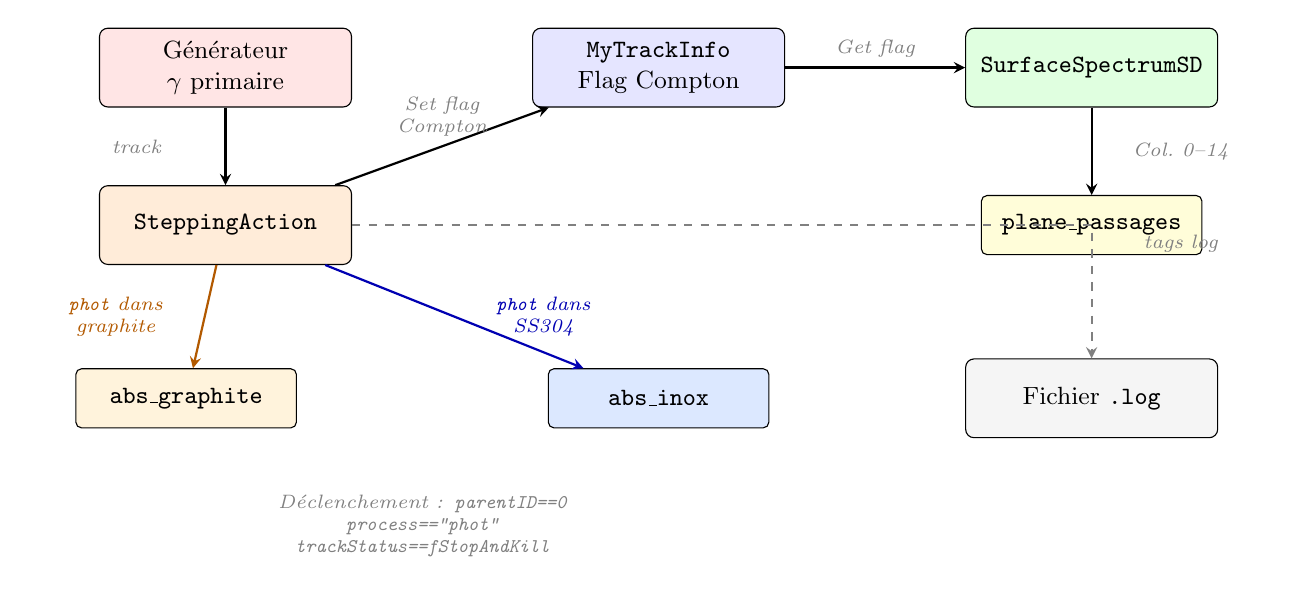
\begin{tikzpicture}[
  box/.style={draw, rounded corners=3pt, minimum height=1cm, minimum width=3.2cm,
              text centered, font=\small, align=center},
  ntuple/.style={draw, rounded corners=2pt, minimum height=0.75cm, minimum width=2.8cm,
              text centered, font=\small\ttfamily, fill=yellow!15, align=center},
  arrow/.style={->, >=stealth, thick},
  note/.style={font=\scriptsize\itshape, text=gray, align=center, text width=2cm},
]

% Source
\node[box, fill=red!10] (gen) at (0, 2) {G\'en\'erateur\\$\gamma$ primaire};

% SteppingAction
\node[box, fill=orange!15] (step) at (0, 0) {\texttt{SteppingAction}};

% MyTrackInfo
\node[box, fill=blue!10] (info) at (5.5, 2) {\texttt{MyTrackInfo}\\Flag Compton};

% SurfaceSpectrumSD
\node[box, fill=green!12] (sd) at (11, 2) {\texttt{SurfaceSpectrumSD}};

% Ntuples
\node[ntuple] (nt_plane) at (11, 0) {plane\_passages};
\node[ntuple, fill=graphite] (nt_graph) at (-0.5, -2.2) {abs\_graphite};
\node[ntuple, fill=inox]     (nt_inox)  at (5.5, -2.2) {abs\_inox};

% Log
\node[box, fill=gray!8] (log) at (11, -2.2) {Fichier \texttt{.log}};

% Flèches
\draw[arrow] (gen) -- node[left, note] {track} (step);
\draw[arrow] (step) -- node[above, note] {Set flag Compton} (info);
\draw[arrow] (info) -- node[above, note] {Get flag} (sd);
\draw[arrow] (sd) -- node[right, note] {Col.\ 0--14} (nt_plane);

\draw[arrow, color=orange!70!black] (step) -- node[left, note, text=orange!70!black] {\texttt{phot} dans\\graphite} (nt_graph);
\draw[arrow, color=blue!70!black] (step) -- node[right, note, text=blue!70!black] {\texttt{phot} dans\\SS304} (nt_inox);

\draw[arrow, dashed, gray] (step) -| node[below right, note] {tags log} (log);

% Condition
\node[note, anchor=north, text width=5cm, align=center] at (2.5, -3.3)
  {D\'eclenchement : \texttt{parentID==0}\\
   \texttt{process=="phot"}\\
   \texttt{trackStatus==fStopAndKill}};

\end{tikzpicture}
\end{center}


% ===================================================================
%  8. TAGS LOG
% ===================================================================
\section{Nouveaux tags dans le fichier \texttt{.log}}

\begin{table}[H]
\centering
\caption{Tags de log ajout\'es pour le suivi des photoabsorptions.}
\label{tab:logtags_abs}

\medskip

\renewcommand{\arraystretch}{1.2}
{\small
\begin{tabular}{llll}
\toprule
\textbf{Tag} & \textbf{Source} & \textbf{Fr\'equence} & \textbf{Contenu} \\
\midrule
\texttt{[STEP][ABS\_GRAPHITE]}
  & \texttt{SteppingAction}
  & 50 premiers, puis 1/10\,000
  & \'Ev\'enement, $E$, position, flag Compton \\[4pt]
\texttt{[STEP][ABS\_INOX]}
  & \texttt{SteppingAction}
  & 50 premiers, puis 1/10\,000
  & \'Ev\'enement, $E$, volume, position, flag Compton \\
\bottomrule
\end{tabular}
}
\end{table}


% ===================================================================
%  9. EXEMPLES D'ANALYSE ROOT
% ===================================================================
\section{Exemples d'analyse ROOT}

\subsection{Ntuple \texttt{abs\_graphite}}

\begin{lstlisting}[style=root]
// Spectre en energie des gamma absorbes dans le graphite
abs_graphite->Draw("ekin_keV")

// Carte (r, z) des absorptions dans le cone
abs_graphite->Draw("z_mm:sqrt(x_mm^2+y_mm^2)",
    "", "COLZ")

// Gamma ayant fait un Compton avant d'etre absorbes
abs_graphite->Draw("ekin_keV",
    "had_compton_in_cone==1")

// Profil z des absorptions directes vs post-Compton
abs_graphite->Draw("z_mm",
    "had_compton_in_cone==0", "", "SAME")
abs_graphite->Draw("z_mm",
    "had_compton_in_cone==1", "", "SAME")
\end{lstlisting}

\subsection{Ntuple \texttt{abs\_inox}}

\begin{lstlisting}[style=root]
// Spectre dans le porte-collimateur uniquement
abs_inox->Draw("ekin_keV",
    "volume==\"logicPorteCollimateur\"")

// Spectre dans l'enveloppe uniquement
abs_inox->Draw("ekin_keV",
    "volume==\"logicEnveloppeGDML\"")

// Carte (x, z) de toutes les absorptions inox
abs_inox->Draw("z_mm:x_mm", "", "COLZ")

// Comparaison porte-collimateur vs enveloppe
abs_inox->Draw("ekin_keV",
    "volume==\"logicPorteCollimateur\"")
abs_inox->Draw("ekin_keV",
    "volume==\"logicEnveloppeGDML\"", "", "SAME")

// Gamma ayant suivi un Compton avant absorption inox
abs_inox->Draw("z_mm",
    "had_compton_in_cone==1")
\end{lstlisting}

\subsection{Analyses crois\'ees}

\begin{lstlisting}[style=root]
// Comptages totaux
cout << "Abs graphite : "
     << abs_graphite->GetEntries() << endl;
cout << "Abs inox     : "
     << abs_inox->GetEntries() << endl;

// Fraction des gamma ayant subi un Compton avant absorption
cout << "Graphite post-Compton : "
     << abs_graphite->GetEntries("had_compton_in_cone==1")
     << " / " << abs_graphite->GetEntries() << endl;

// Rapport avec les transmis au ScorePlane
cout << "Transmis directs     : "
     << plane_passages->GetEntries(
        "pdg==22 && is_secondary==0 && compton_in_cone==0")
     << endl;
cout << "Transmis Compton     : "
     << plane_passages->GetEntries(
        "pdg==22 && is_secondary==0 && compton_in_cone==1")
     << endl;
\end{lstlisting}


% ===================================================================
%  10. COMPATIBILITE
% ===================================================================
\section{Compatibilit\'e et remarques}

\begin{itemize}[nosep]
\item \textbf{Pr\'erequis :} les modifications \texttt{MyTrackInfo} (flag Compton)
      doivent \^etre en place pour que les colonnes \texttt{had\_compton\_in\_cone}
      et \texttt{n\_compton\_in\_cone} soient renseign\'ees.
      Sans ces modifications, ces colonnes vaudront toujours~0.
\item \textbf{Ntuples existants :} les 5 ntuples de passages (plans 1--5)
      restent inchang\'es dans leur structure.
\item \textbf{Taille du fichier ROOT :} l'impact d\'epend du nombre d'absorptions.
      Pour 50M \'ev\'enements, on attend $\sim$30M entr\'ees dans \texttt{abs\_inox}
      et $\sim$17M dans \texttt{abs\_graphite} (d'apr\`es les bilans
      \texttt{[LOSS][BY-MAT]} pr\'ec\'edents),
      soit $\sim$200--300~Mo suppl\'ementaires.
\item \textbf{Multi-thread :} le remplissage utilise \texttt{G4AnalysisManager}
      qui g\`ere en interne la s\'erialisation des ntuples en mode MT.
      Les compteurs de log sont \texttt{static} dans des fonctions appel\'ees
      par thread (pas de race condition sur le compteur de log car l'ordre
      d'affichage n'est pas critique).
\item \textbf{Recompilation :} un \texttt{make} incr\'emental suffit
      (3 fichiers modifi\'es).
\end{itemize}


% ===================================================================
%  RECAPITULATIF GLOBAL
% ===================================================================
\section*{R\'ecapitulatif global des modifications (les deux synth\`eses)}

Au total, 6 fichiers ont \'et\'e modifi\'es :

\begin{table}[H]
\centering
\renewcommand{\arraystretch}{1.2}
{\small
\begin{tabular}{llcc}
\toprule
\textbf{Fichier} & \textbf{R\'ep.} & \textbf{Modif.\ 1} & \textbf{Modif.\ 2} \\
 & & \textit{(Compton)} & \textit{(Photoabs.)} \\
\midrule
\texttt{MyTrackInfo.hh}           & \texttt{include/} & $\checkmark$ & --- \\
\texttt{MyTrackInfo.cc}           & \texttt{src/}     & $\checkmark$ & --- \\
\texttt{SteppingAction.cc}        & \texttt{src/}     & $\checkmark$ & $\checkmark$ \\
\texttt{SurfaceSpectrumSD.cc}     & \texttt{src/}     & $\checkmark$ & --- \\
\texttt{AnalysisManagerSetup.hh}  & \texttt{include/} & ---          & $\checkmark$ \\
\texttt{AnalysisManagerSetup.cc}  & \texttt{src/}     & $\checkmark$ & $\checkmark$ \\
\bottomrule
\end{tabular}
}
\end{table}


\end{document}
